% Requires \usepackage{algorithm} and \usepackage{algpseudocode}.

% \section{CriticOPD: Restoring Recoverability with Critique}
% \label{sec:method}

% We show in Section~\ref{sec:diagnosis} that after the student errs, the teacher can no longer continue correctly but can still point out the errors of the student. We introduce CriticOPD (Figure~\ref{fig:pipeline}) to restore correct reasoning behaviors following critique. The teacher critiques an incorrect solution of the student, and the student rewrites its solution from the last error with the critique in context. The teacher scores the rewrite with the critique in its context, while the student learns from the sequence without the critique. Section~\ref{sec:privileged} explains why the critique restores recoverability, Section~\ref{sec:rewrite} describes the critique and the rewrite, and Section~\ref{sec:fbd} gives the objective.

% \subsection{Critique as Privileged Information}
% \label{sec:privileged}

% For an incorrect rollout $y$ of the student, the teacher reads the problem $x$, the reference answer, and $y$, and produces a critique $c$, which states where the errors are and how to fix them. Conditioned on $c$, the next-token distribution of the teacher becomes $\pi_T(\cdot \mid s, c)$, and we denote by $V^T(s, c)$ its probability of reaching a correct answer from a state $s$. After the critiqued position, CriticOPD replaces the recoverability $V^T(s)$ of the teacher with $V^T(s, c)$ in the supervision.



% % \begin{figure}[t]
% % \centering
% % 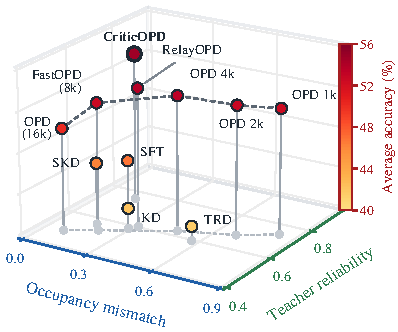
\includegraphics[width=\columnwidth]{figures/fig_mismatch.pdf}
% % \caption{Occupancy mismatch and teacher reliability on the states that each method supervises, and the average accuracy of the Qwen3-1.7B student.}
% % \label{fig:mismatch-reliability}
% % \end{figure}

% \noindent\textbf{The rewrite restores the recoverability of the teacher.}
% Figure~\ref{fig:rewrite-effect}(a) measures the success rates of the teacher and the student from each cut point, as in Section~\ref{sec:diagnosis}, on the original rollout (dashed), which OPD trains on, and on the rewrite (solid), which CriticOPD trains on. On the original rollout, the success rate of the teacher falls from 0.31 at the cut point to 0.14, and that of the student falls from 0.11 to 0.04. On the rewrite, the success rate of the teacher stays between 0.40 and 0.28, and that of the student rises from 0.11 to 0.16, because the rewrite corrects the earlier errors at its start. A generic hint does not raise the success rate of the student, so this improvement comes from the content of the critique. The rewrite does not fully restore the recoverability of the teacher, but at every position after the cut point, its states are more recoverable for both the teacher and the student than those of the original rollout.

% \begin{figure}[t]
% \centering
% \includegraphics[width=\columnwidth]{figures/fig_4.pdf}
% \caption{(a) Success rates around the cut point on the original rollout (dashed) and the rewrite (solid), on which the teacher sees the critique. (b) Token positions of the prefixes that each method trains on and of the inference prefixes, with their total variation distance.}
% \label{fig:rewrite-effect}
% \end{figure}

% The student therefore imitates $\pi_T(\cdot \mid s, c)$ instead of $\pi_T(\cdot \mid s)$. The critique is available during training but not at inference, which is the setting of learning with privileged information \citep{vapnik2009lupi}: the teacher provides the target with the critique, and the student approaches it without the critique \citep{lopezpaz2016unifying}. The student thus learns to make from the prefix alone the correction that it would make if the error were pointed out. OPD is the special case of an empty critique, which CriticOPD keeps for correct rollouts.

% \subsection{Critique and Rewrite}
% \label{sec:rewrite}

% \noindent\textbf{Critique.}
% We split the solution of the student into numbered paragraphs and give them to the teacher with the problem and the reference answer. The teacher lists at most five errors in their order of appearance, each with the paragraph index, the quoted sentence, and a fix of at most three sentences (Appendix~\ref{app:prompts}). The reference answer lets the teacher critique problems that it cannot solve itself. If the teacher finds no error, it returns \textsc{None}, and the rollout is trained with standard OPD. We discard items that are incomplete.

% \noindent\textbf{Cut point.}
% The student keeps its prefix up to the paragraph of the last retained error and discards the rest. The rewrite therefore starts from a state that contains all errors that the critique points out, which is the kind of state from which the teacher cannot recover in Section~\ref{sec:diagnosis} and which the student reaches at inference. The correct work before the cut point is kept and is not generated again. Figure~\ref{fig:rewrite-effect}(b) shows that the student keeps a median of 73\% of the original rollout, and the rewrite replaces 33\% of its tokens on average.

% \noindent\textbf{Rewrite.}
% The student appends the critique to the kept prefix and generates a new suffix itself. The student, rather than the teacher, writes the suffix because the supervision of OPD is valid only on tokens that the student samples: a suffix that the teacher writes depends on knowledge that the student lacks, and training on it would bring back the distribution shift of training on teacher text. The critique changes who scores the suffix, not who writes it. In the example of Figure~\ref{fig:example}, the rewrite returns to the critiqued paragraph, corrects the error, and continues to the answer.

% \begin{figure*}[t]
% \centering
% 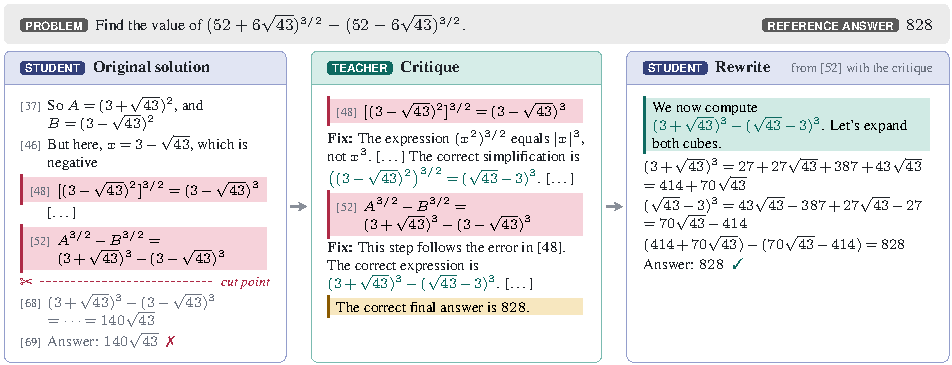
\includegraphics[width=\textwidth]{figures/fig_example.pdf}
% \caption{An example of critique-guided rewriting. Left: the original solution, with the critiqued paragraphs marked. Middle: the critique, which quotes each erroneous sentence, gives a fix, and ends with the reference answer. Right: the suffix that the student writes from the last error with the critique.}
% \label{fig:example}
% \end{figure*}

% \subsection{Feedback Distillation}
% \label{sec:fbd}

% Let $p$ denote the kept prefix and $y' = (y'_1, \dots, y'_m)$ the new suffix. The training sequence concatenates $p$ and $y'$ without the critique, and each token of the suffix receives the advantage
% \begin{equation}
% \begin{split}
% A^{\mathrm{fb}}_t ={}& \log \pi_T(y'_t \mid x, p, c, y'_{<t}) \\
% &- \log \pi_\theta(y'_t \mid x, p, y'_{<t}),
% \end{split}
% \label{eq:fb}
% \end{equation}
% in which the teacher scores with the critique and the student does not see it. The prefix receives no loss, because it contains the errors and its states are those from which the teacher cannot recover. We denote this loss by $\mathcal{L}_{\mathrm{fb}}$. The objective of CriticOPD sums the OPD loss on correct rollouts and $\mathcal{L}_{\mathrm{fb}}$ on incorrect rollouts, and Algorithm~\ref{alg:criticopd} summarizes one training step.

% \begin{algorithm}[t]
% \caption{One training step of CriticOPD}
% \label{alg:criticopd}
% \begin{algorithmic}[1]
% \Require student $\pi_\theta$, teacher $\pi_T$, problems with reference answers $\{(x, a)\}$
% \For{each problem $(x, a)$}
%     \State Sample $y \sim \pi_\theta(\cdot \mid x)$
%     \If{$y$ reaches $a$}
%         \State Add the OPD loss on $y$ \Comment{Eq.~\eqref{eq:adv}}
%     \Else
%         \State $c \gets$ critique of $y$ by $\pi_T$ given $x$ and $a$, without incomplete items
%         \If{$c = \textsc{None}$}
%             \State Add the OPD loss on $y$
%         \Else
%             \State $p \gets$ prefix of $y$ up to the paragraph of the last error in $c$
%             \State Sample $y' \sim \pi_\theta(\cdot \mid x, p, c)$
%             \State Add the loss on $y'$ with $\pi_T(\cdot \mid x, p, c, y'_{<t})$ \Comment{Eq.~\eqref{eq:fb}; no loss on $p$}
%         \EndIf
%     \EndIf
% \EndFor
% \State Update $\theta$ with the summed loss
% \end{algorithmic}
% \end{algorithm}

\section{CriticOPD: Restoring Recoverability with Critique}
\label{sec:method}

Section~\ref{sec:diagnosis} shows that after the student errs, the teacher may fail to continue correctly but can still recognize the errors. We therefore build training sequences that the student writes from the states that it reaches at inference, which adds little occupancy mismatch, and on which the teacher supervision is reliable. Section~\ref{sec:rewrite} builds these sequences and measures the recoverability of the teacher on them, and Section~\ref{sec:fbd} gives the training objective.

\subsection{Critique and Rewrite}
\label{sec:rewrite}

\noindent\textbf{Trigger.}
The student generates a rollout $y$ for each problem $x$ with the prompt $\mathcal{P}_{\text{train}}$. Incorrect rollouts and those reaching the length limit without an answer are sent for critique and rewriting. Correct rollouts are trained with standard OPD.

\noindent\textbf{Critique.}
The teacher serves as the critic. It receives the problem, the reference answer, and the solution of the student in numbered paragraphs, and it lists the errors in the solution (prompts $\mathcal{P}_{\text{critic}}$ and $\mathcal{P}_{\text{critic-user}}$ in Appendix~\ref{app:prompts-method}). Each error contains the index of its paragraph, the erroneous sentence, and a short fix. We combine these errors and the reference answer into the critique $c$. The reference answer lets the teacher critique problems that it cannot solve. If the critique contains no complete error, the rollout is trained with standard OPD.

\noindent\textbf{Cut point.}
The student keeps its prefix through the paragraph of the last error in the critique and discards the rest. The discarded part starts at position $\tau$, so the retained prefix is $h_\tau=(x,y_{<\tau})$. This prefix contains all errors in the critique, so the rewrite starts from the erroneous states where teacher recoverability declines (Section~\ref{sec:diagnosis}).

\noindent\textbf{Rewrite.}
The student appends the critique $c$ to the retained prefix with the prompt $\mathcal{P}_{\text{fb}}$ and generates a new suffix, which gives the revised rollout $\tilde{y}$. The tokens before $\tau$ are unchanged, $\tilde{y}_{<\tau}=y_{<\tau}$, and the student samples the suffix with the critique in its context. Unlike teacher takeover, the student writes every token of the training sequence. In Figure~\ref{fig:example}, the critique identifies two errors, and the student rewrites from the last one to reach the correct answer.

\begin{figure*}[t]
\centering
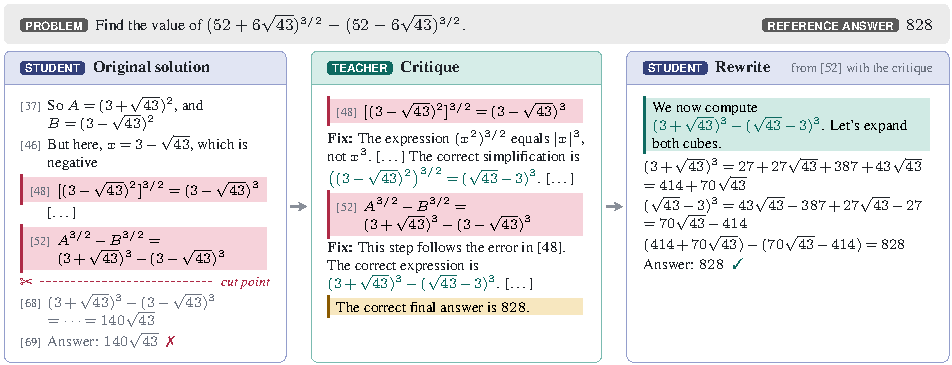
\includegraphics[width=\textwidth]{figures/fig_example.pdf}
\caption{An example of critique-guided rewriting. Left: the original solution, with the critiqued paragraphs marked. Middle: the critique, which quotes each erroneous sentence, gives a fix, and ends with the reference answer. Right: the suffix that the student writes from the last error with the critique.}
\label{fig:example}
\end{figure*}

\noindent\textbf{Recoverability on the rewrite.}
We test whether the teacher is more reliable on the rewrite than on the original rollout. As in Section~\ref{sec:diagnosis}, we estimate recoverability as the fraction of correct answers among eight continuations from each prefix. The test uses the student after 80 steps of OPD and the 161 incorrect rollouts of Appendix~\ref{app:rewrite-analysis}. We critique and cut each rollout as CriticOPD does, and the student writes a rewrite with the critique. This student is not trained with CriticOPD, so the rewrite differs from the original rollout only through the critique. Figure~\ref{fig:rewrite-effect} compares recoverability after the cut point on the two sequences. On the original rollout, the teacher continues from the prefix of the student, and on the rewrite, the teacher continues with the critique in its context. At 75\% of the continuation, the recoverability of the teacher is 0.14 on the original rollout and 0.67 on the rewrite, and the success rate of the student without the critique rises from 0.03 to 0.16.

\begin{figure}[t]
\centering
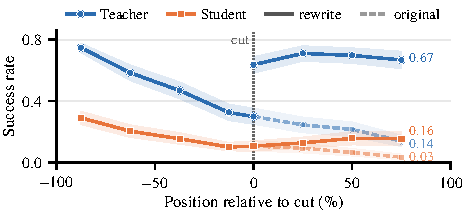
\includegraphics[width=\columnwidth]{figures/fig_rewrite.pdf}
\caption{Recoverability of the teacher and the student on original rollouts (dashed) and critique-guided rewrites (solid), plotted against the position relative to the cut point. On the rewrite, the teacher sees the critique, and the student does not.}
\label{fig:rewrite-effect}
\end{figure}

\subsection{Training Objective}
\label{sec:fbd}
\label{sec:privileged}

\noindent\textbf{Standard OPD.}
For correct rollouts and rollouts without a valid critique, we minimize the reverse KL $\mathcal{L}_{\mathrm{OPD}}(y)=\sum_{t=1}^{|y|}\mathrm{KL}\big(\pi_\theta(\cdot\mid h_t)\,\|\,\pi_T(\cdot\mid h_t)\big)$ at each student-generated prefix $h_t$ with the sampled-token advantage in Equation~\eqref{eq:adv}.

\noindent\textbf{Feedback distillation.}
For rollouts with a valid critique, we train on the revised sequence $\tilde{y}$. Let $\tilde{h}_t=(x,\tilde{y}_{<t})$ denote its prefix without the critique. The teacher scores the rewrite with $c$ in its context, while the student does not see it:
\begin{equation}
\mathcal{L}_{\mathrm{fb}}(\tilde{y};c)
=
\sum_{t=\tau}^{|\tilde{y}|}
\mathrm{KL}\left(
\pi_\theta(\cdot\mid\tilde{h}_t)
\,\big\|\,
\pi_T(\cdot\mid\tilde{h}_t,c)
\right).
\label{eq:fb-loss}
\end{equation}
Only the rewritten suffix receives supervision, since the retained prefix contains errors at states where the teacher has low recoverability. As in OPD, each suffix token receives the sampled-token advantage
\begin{equation}
A_t^{\mathrm{fb}}
=
\log\pi_T(\tilde{y}_t\mid\tilde{h}_t,c)-\log\pi_\theta(\tilde{y}_t\mid\tilde{h}_t).
\label{eq:fb}
\end{equation}
The suffix is sampled with the critique, whereas the log-probabilities of the student are computed without it, so this update is a surrogate rather than an unbiased gradient of Equation~\eqref{eq:fb-loss}.

\noindent\textbf{Overall objective.}
CriticOPD minimizes $\mathcal{L}_{\mathrm{ours}}=\mathcal{L}_{\mathrm{OPD}}+\mathcal{L}_{\mathrm{fb}}$, where each loss sums over its rollouts in the batch and each rollout enters exactly one term. Compared with OPD, the teacher target changes from $\pi_T(\cdot\mid h_t)$ to $\pi_T(\cdot\mid\tilde{h}_t,c)$, under which the teacher is much more recoverable (Section~\ref{sec:rewrite}). The student learns without the critique and needs no feedback at inference. Algorithm~\ref{alg:criticopd} in Appendix~\ref{app:config} summarizes one training step.
